\begin{tcolorbox}
Die Produktfunktionen beschreiben jede einzelne Funktion des Produkts mittels Anwendungsfalldiagrammen und Anwendungsfalltabellen.
Diese sollen möglichst ausschlaggebend für das zu entwickelnde System sein und nicht simple Produktfunktionen wie z.B. Login, Account erstellen, Gruppe beitreten, Passwort ändern oder ähnliches zeigen.
\autoref{fig:anwendungsfall-app-tabelle-xx-1} stellt eine exemplarische Tabelle für die Beschreibung eines Anwendungsfalls dar. Stil und Formatierung sind variabel. Nicht jede Zelle muss immer gefüllt sein.
\\\\
In  Tabelle~\autoref{fig:akteur-tabelle} werden alle auftretenden Akteure beschrieben.


\end{tcolorbox}

\begin{figure}[h]
	\centering
	
	\begin{tabularx}{\textwidth}{ p{.2\textwidth} | p{.2\textwidth} | X }
		\textbf{Akteur} & \textbf{Beschreibung} & \textbf{Verwendet in Anwendungsfall} \\ \hline
		Informatiker & Programmiert tolle Sachen & Programmieren, Kaffee trinken, Schlafen
	\end{tabularx}
	
	\caption{Beschreibung der Akteure}
	\label{fig:akteur-tabelle}
\end{figure}

%%%%%%%%%%%%%%%
%% Eigene Arbeit %%
%%%%%%%%%%%%%%%

%%%%%%%%%%%%%%%
%% Anwendungsfall 1 %%
%%%%%%%%%%%%%%%

\section{Anwendungsfalldiagramm - App}

\begin{figure}[h]
	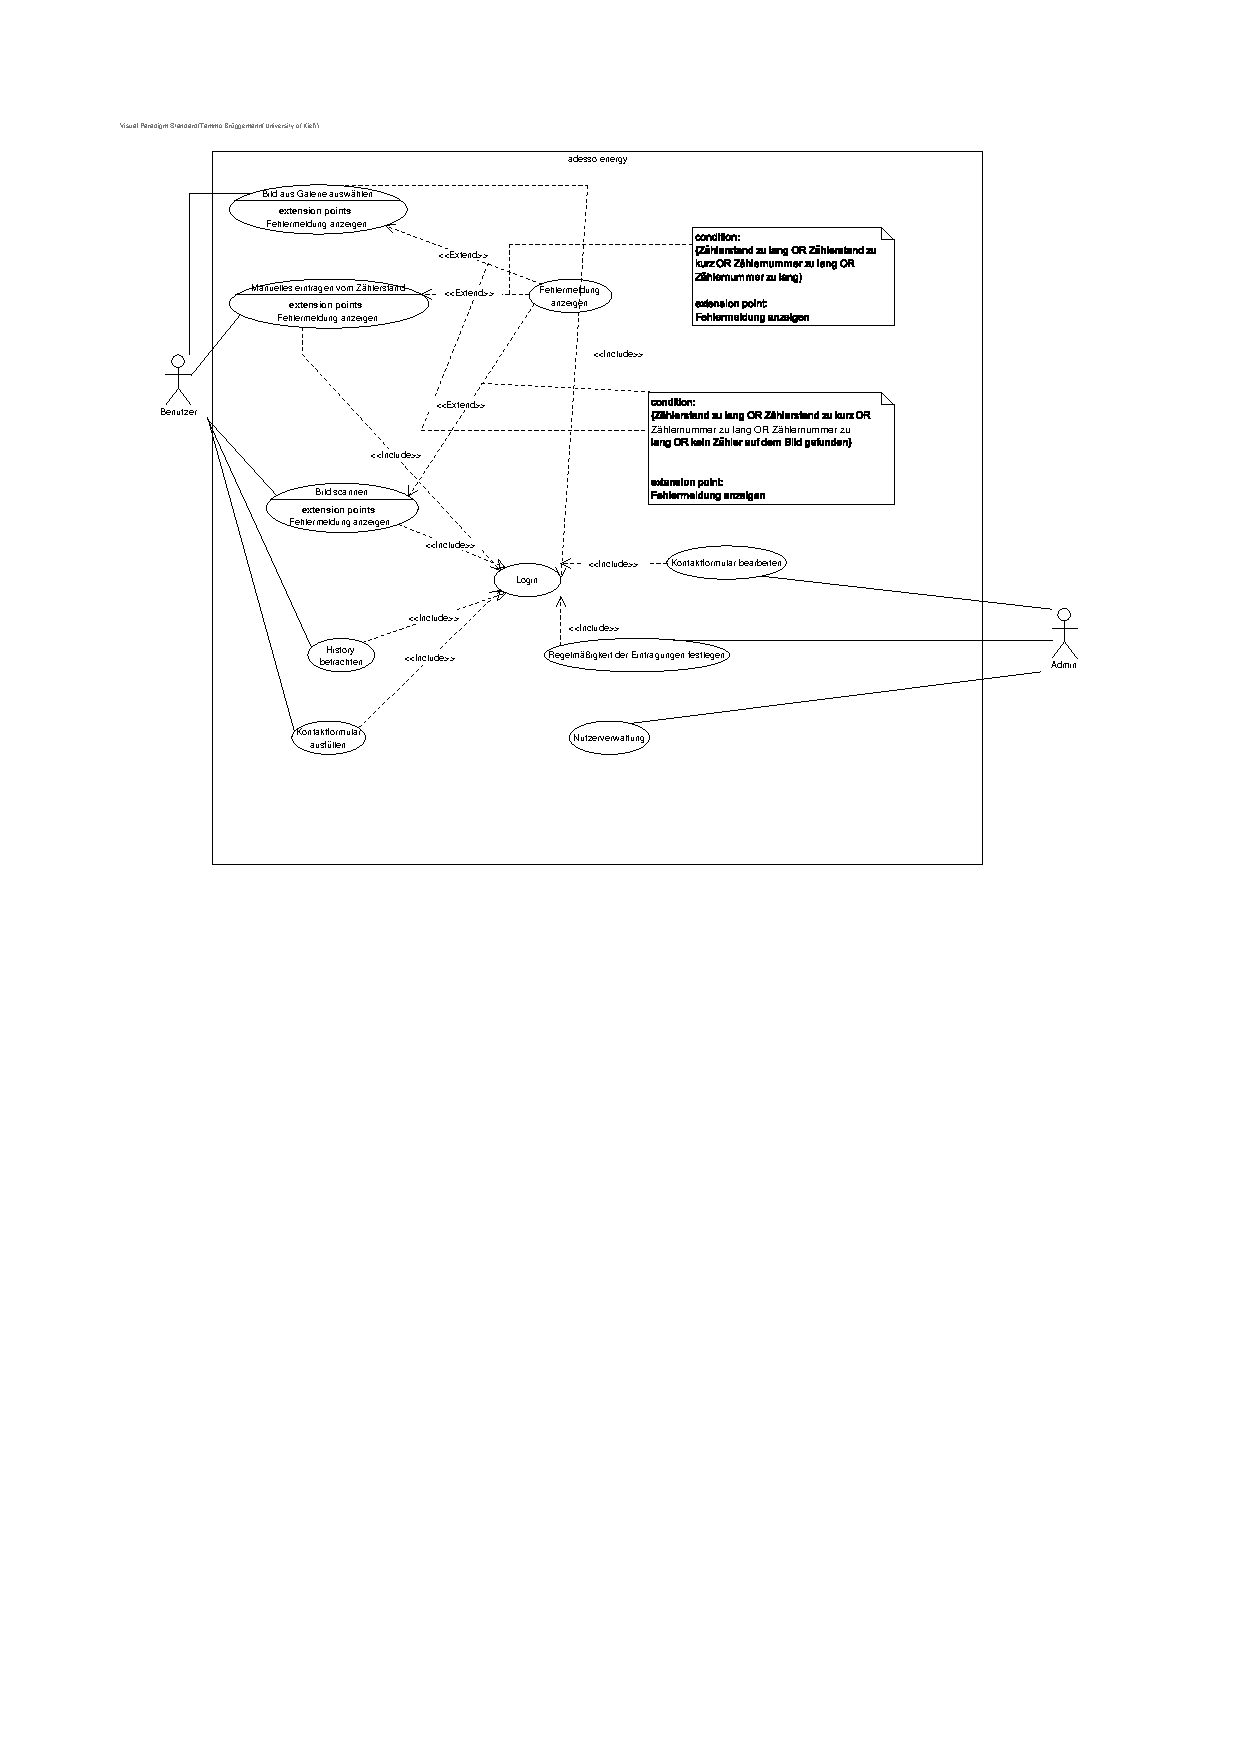
\includegraphics[width=20cm]{./img/mustCase}
%	\centering
%	\missingfigure{Anwendungsfalldiagramm - App}		
%	\caption{Anwendungsfalldiagramm - App}
%	\label{fig:anwendungsfalldiagramm-app}
\end{figure}

\newpage

\begin{figure}[h]
	\centering
	\begin{tabularx}{\textwidth}{ X | X }
		\textbf{Anwendungsfall ID} & 1 \\ \hline
		\textbf{Anwendungsfallname} & Bild hochladen  - Foto \\ \hline
		\textbf{Initiierender Akteur} & Benutzer \\ \hline
		\textbf{Weitere Akteure} & - \\ \hline
		\textbf{Kurzbeschreibung} & Der Benutzer macht in der App ein Foto und lädt dieses hoch.   \\ \hline
		\textbf{Vorbedingungen} & 
		\begin {itemize}
			\item Eingeloggt sein. 
			\item Hauptbildschirm geöffnet.
			\item Auf Kamera FAB gedrückt.
		\end{itemize} \\ \hline
		\textbf{Nachbedingungen} & Zählerstand wurde erkannt und eingetragen.  \\ \hline
		\textbf{Ablauf} &
		\begin{enumerate}
			\item Benutzer macht Foto.
			\item Benutzer bestätigt Senden des Fotos.
			\item Azure wertet Bild aus.
			\item Erkannte Zählernummer und Zählerstand werden angezeigt.
			\item Benutzer bestätigt Korrektheit der Zählernummer und des Zählerstandes.
		\end{enumerate} \\ \hline
		\textbf{Alternative} &
		\begin{enumerate}
			\item Benutzer macht Foto.
			\item Benutzer bestätigt Senden des Fotos.
			\item Azure wertet Bild aus.
			\item Erkannte Zählernummer und Zählerstand werden angezeigt.
			\item Benutzer bricht Aktion ab.
		\end{enumerate} \\ &
		\begin{enumerate}
			\item Benutzer macht Foto.
			\item Benutzer bestätigt Senden des Fotos.
			\item Azure wertet Bild aus.
			\item Erkannte Zählernummer und Zählerstand werden angezeigt.
			\item Benutzer verbessert Eingabe manuell.
		\end{enumerate} \\


	\end{tabularx}
\end{figure}

\begin{figure}[h]
	\centering
	\begin{tabularx}{\textwidth}{ X | X }
	 \hline
		\textbf{Ausnahme} &
		\begin{enumerate}
			\item Benutzer macht Foto.
			\item Benutzer bestätigt Senden des Fotos.
			\item Azure wertet Bild aus
			\item Fehler beim Auslesen der Zählernummer oder des Zählerstandes.
			\item $\lbrack$ Use-Case: Fehlermeldung wird angezeigt $\rbrack$
		\end{enumerate} \\ &
		\begin{enumerate}
			\item Benutzer macht Foto.
			\item Benutzer bestätigt Senden des Fotos.
			\item Azure wertet Bild aus
			\item Zählernummer und Zählerstand wurden erkannt, aber mindestens einer der beiden Werte ist unzulässig. (falsches Format)
			\item $\lbrack$ Use-Case: Fehlermeldung wird angezeigt $\rbrack$
		\end{enumerate} \\  &
		\begin{enumerate}
			\item Benutzer macht Foto.
			\item Benutzer bestätigt Senden des Fotos.
			\item Es liegt ein Serverfehler vor.
			\item Die App zeigt eine 'Bitte versuche es nochmal'-Meldung.
		\end{enumerate} \\ \hline &
		\begin{enumerate}
			\item Benutzer macht Foto.
			\item Benutzer bestätigt Senden des Fotos.
			\item Nutzer hat keine Internetverbindung.
			\item Die App zeigt eine 'Du bist offline'-Meldung.
		\end{enumerate} \\ \hline
		\textbf{Benutzte Anwendungsfälle} & Fehlermeldung wird angezeigt \\ \hline
		\textbf{Spezielle Anforderungen} & - \\ \hline
		\textbf{Annahmen} & -
	\end{tabularx}
	\caption{Anwendungsfall Bildhochladen-1}
	\label{fig:anwendungsfall-server-tabelle-xx-1}
\end{figure}

\newpage

\begin{figure}[h]
	\centering
	\begin{tabularx}{\textwidth}{ X | X }
		\textbf{Anwendungsfall ID} & 2 \\ \hline
		\textbf{Anwendungsfallname} & Zählerstand manuell eingeben. \\ \hline
		\textbf{Initiierender Akteur} & Benutzer \\ \hline
		\textbf{Weitere Akteure} & - \\ \hline
		\textbf{Kurzbeschreibung} & Der Benutzer hat, neben dem Abfotografieren des Zählerstandes, auch noch die Möglichkeit den Zählerstand manuell 									einzugeben.  \\ \hline
		\textbf{Vorbedingungen} & 
		\begin {itemize}
			\item Eingeloggt sein. 
			\item Hauptbildschirm geöffnet.
			\item Zähler auswählen.
			\item Auf Button 'Neue manuelle Eingabe' drücken.
		\end{itemize}\\ \hline
		\textbf{Nachbedingungen} & Zählerstand wurde eingetragen.  \\ \hline
		\textbf{Ablauf} &
		\begin{enumerate}
			\item Benutzer überprüft ob angezeigte Zählernummer mit der Zählernummer des ausgewählten Zählers übereinstimmt.
			\item Benutzer gibt Zählerstand ein.
			\item Benutzer bestätigt Zählerstand.
		\end{enumerate} \\ \hline
		\textbf{Alternative} & - \\ \hline
		\textbf{Ausnahme} &
		\begin{enumerate}
			\item Benutzer überprüft ob angezeigte Zählernummer mit der Zählernummer des ausgewählten Zählers übereinstimmt.
			\item Benutzer bricht Aktion ab.
		\end{enumerate}  \\  &
		\begin{enumerate}
			\item Benutzer überprüft ob angezeigte Zählernummer mit der Zählernummer des ausgewählten Zählers übereinstimmt.
			\item Benutzer gibt Zählerstand ein.
			\item Benutzer bestätigt Zählerstand.
			\item Zählerstand ist unzulässig. (falsches Format)
			\item 'Dieser Wert ist unzulässig. Bitte erneut eingeben'-Meldung wird angezeigt. 
		\end{enumerate} \\


	\end{tabularx}
\end{figure}

\begin{figure}[h]
	\centering
	\begin{tabularx}{\textwidth}{ X | X }
	&
		\begin{enumerate}
			\item Benutzer überprüft ob angezeigte Zählernummer mit der Zählernummer des ausgewählten Zählers übereinstimmt.
			\item Benutzer gibt Zählerstand ein.
			\item Benutzer bestätigt Zählerstand.
			\item Es liegt ein Serverfehler vor.
			\item Die App zeigt eine 'Bitte versuche es nochmal'-Meldung. 
		\end{enumerate} \\  &
		\begin{enumerate}
			\item Benutzer überprüft ob angezeigte Zählernummer mit der Zählernummer des ausgewählten Zählers übereinstimmt.
			\item Benutzer gibt Zählerstand ein.
			\item Benutzer bestätigt Zählerstand.
			\item Nutzer hat keine Internetverbindung.
			\item Die App zeigt eine 'Du bist offline'-Meldung.
		\end{enumerate}  \\ \hline
		\textbf{Benutzte Anwendungsfälle} & - \\ \hline
		\textbf{Spezielle Anforderungen} & - \\ \hline
		\textbf{Annahmen} & -
	\end{tabularx}
	\caption{Zählerstand manuell eingeben.}
	\label{fig:anwendungsfall-server-tabelle-xx-1}
\end{figure}

\newpage

\begin{figure}[h]
	\centering
	\begin{tabularx}{\textwidth}{ X | X }
		\textbf{Anwendungsfall ID} & 3 \\ \hline
		\textbf{Anwendungsfallname} & Fehlermeldung anzeigen. \\ \hline
		\textbf{Initiierender Akteur} & Benutzer \\ \hline
		\textbf{Weitere Akteure} & - \\ \hline
		\textbf{Kurzbeschreibung} & Falls beim Auslesen eines Bildes ein Problem auftritt, wird eine dem User eine Fehlermeldung angezeigt.   \\ \hline
		\textbf{Vorbedingungen} & 
		\begin {itemize}
			\item Eingeloggt sein. 
			\item Hauptbildschirm geöffnet.
			\item Bild wurde hochgeladen.
			\item Azure konnte Bild nicht auswerten.
		\end{itemize}\\ \hline
		\textbf{Nachbedingungen} & - \\ \hline
		\textbf{Ablauf} &
		\begin{enumerate}
			\item Meldung 'Scan nicht erfolgreich' wird angezeigt
			\item Benutzer drückt auf 'Neuer Scan"
			\item $\lbrack$ Use-Case: Bild hochladen - Foto $\rbrack$
		\end{enumerate} \\ \hline
		\textbf{Alternative} & 
		\begin{enumerate}
			\item Meldung 'Scan nicht erfolgreich' wird angezeigt
			\item Benutzer drückt auf 'Abbrechen'
			\item Benutzer ist wieder auf Startbildschirm
		\end{enumerate} \\ \hline
		\textbf{Ausnahme} & -   \\ \hline
		\textbf{Benutzte Anwendungsfälle} & Bild hochladen - Foto \\ \hline
		\textbf{Spezielle Anforderungen} & - \\ \hline
		\textbf{Annahmen} & -
	\end{tabularx}
	\caption{Fehlermeldung anzeigen.}
	\label{fig:anwendungsfall-server-tabelle-xx-1}
\end{figure}



